\documentclass{tufte-handout}

%\geometry{showframe}% for debugging purposes -- displays the margins

\usepackage{amsmath}

% Set up the images/graphics package
\usepackage{graphicx}
\setkeys{Gin}{width=\linewidth,totalheight=\textheight,keepaspectratio}
\graphicspath{{graphics/}}

\title{Conceptual framework}
% \author[Tobi]{Tobias Bretschneider}
% \date{}  % if the \date{} command is left out, the current date will be used

% The following package makes prettier tables.  We're all about the bling!
\usepackage{booktabs}

% The units package provides nice, non-stacked fractions and better spacing
% for units.
\usepackage{units}

% The fancyvrb package lets us customize the formatting of verbatim
% environments.  We use a slightly smaller font.
\usepackage{fancyvrb}
\fvset{fontsize=\normalsize}

% Small sections of multiple columns
\usepackage{multicol}

% Provides paragraphs of dummy text
\usepackage{lipsum}

% These commands are used to pretty-print LaTeX commands
\newcommand{\doccmd}[1]{\texttt{\textbackslash#1}}% command name -- adds backslash automatically
\newcommand{\docopt}[1]{\ensuremath{\langle}\textrm{\textit{#1}}\ensuremath{\rangle}}% optional command argument
\newcommand{\docarg}[1]{\textrm{\textit{#1}}}% (required) command argument
\newenvironment{docspec}{\begin{quote}\noindent}{\end{quote}}% command specification environment
\newcommand{\docenv}[1]{\textsf{#1}}% environment name
\newcommand{\docpkg}[1]{\texttt{#1}}% package name
\newcommand{\doccls}[1]{\texttt{#1}}% document class name
\newcommand{\docclsopt}[1]{\texttt{#1}}% document class option name

\usepackage{tikz}
\usetikzlibrary{arrows.meta, positioning, fit, backgrounds}

\begin{document}

\maketitle% this prints the handout title, author, and date

% \begin{abstract}
% \noindent This document describes the Tufte handout \LaTeX\ document style.
% It also provides examples and comments on the style's use.  Only a brief
% overview is presented here; for a complete reference, see the sample book.
% \end{abstract}

%\printclassoptions

\section{Introduction}

We set out the conceptual framework that will allow us to unify the various ideas
presented. First we clarify the difference between the probabilistic and the
deterministic view of Neural nets, then we show how various notions of metrics defined
on the ``output'' will in a sense give recognisable objects when pulled back either to
the parameter space, or the data space.

\begin{figure}[h!]
%  \checkparity This is an \pageparity\ page.%
  \caption{Probabilistic vs. Deterministic view of neural nets.
}
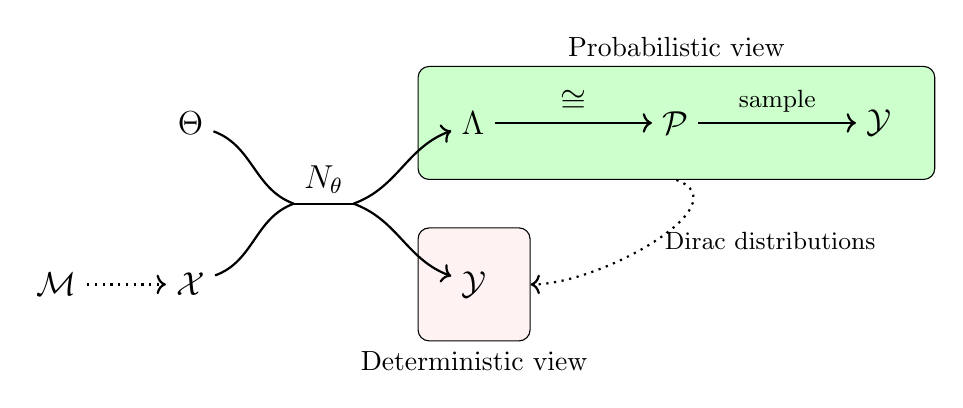
\begin{tikzpicture}[
    thick,
    node distance=2.5cm,
    every node/.style={font=\large},
    box/.style={draw, rounded corners, fill=#1!20, inner sep=10pt},
    arrow/.style={->, thick},
    dashedarrow/.style={->, dashed, thick},
    dottedarrow/.style={->, dotted, thick}
]

% Nodes
\node (M) {$\mathcal{M}$};
\node[right=1cm of M] (X) {$\mathcal{X}$};
\node[above=1.5cm of X] (Theta) {$\Theta$};

\node[above right=0.75cm and 1cm of X] (Ntheta) {$N_\theta$};

\node[above right=1.5cm and 3cm of X] (Lambda) {$\Lambda$};
\node[right=2cm of Lambda] (P) {$\mathcal{P}$};
\node[right=2cm of P] (PY) {$\mathcal{Y}$};

\node[right=3cm of X] (Y) {$\mathcal{Y}$};

% Arrows into N_theta
\draw (X) to[out=20, in=-160] (Ntheta.south west);
\draw (Theta) to[out=-20, in=160] (Ntheta.south west);

% Line below N_theta
\draw (Ntheta.south west) -- (Ntheta.south east);

\draw[arrow] (Ntheta.south east) to[out=20, in=-160] (Lambda);
\draw[arrow] (Ntheta.south east) to[out=-20, in=160] (Y);

\draw[arrow] (Lambda) -- node[midway, above] {$\cong$} (P);
\draw[arrow] (P) -- node[midway, above] {\small sample} (PY);

% Dotted arrow from M to X
\draw[dottedarrow] (M) -- (X);

% --- Boxes (background layer so they sit behind) ---
\begin{scope}[on background layer]

% Probabilistic (green)
\node[draw, rounded corners, fill=green!20, inner sep=12pt,
      fit=(Lambda) (P) (PY),
      label={[font=\normalsize]above:Probabilistic view}] (probbox) {};

% Deterministic (pink)
\node[draw, rounded corners, fill=pink!20, inner sep=12pt,
      fit=(Y),
      label={[font=\normalsize]below:Deterministic view}] (detbox) {};

\end{scope}

% Curved dotted arrow between boxes
\draw[dottedarrow]
    (probbox.south) to[out=-20, in=0]
    node[midway, right] {\small Dirac distributions}
    (detbox.east);

\end{tikzpicture}
  \label{fig:prob-vs-det}
  %\zsavepos{pos:textfig}
  %\setfloatalignment{b}
\end{figure}

\section{Probabilistic vs. Deterministic}

On the one hand we can get our neural net, $N_\theta$ to directly output the quantity of
interest (the deterministic view), alternatively we output parameters, $\lambda \in
\Lambda$, which correspond to a probability distribution from which we can sample.

The deterministic view point is used by:
\begin{itemize}
    \item All papers from the AGOP community\cite[-4cm]{Radhakrishnan2024,DePavia2025}; and,
    \item work on representation similarity analysis\cite{Cayco_Gajic2026}.
\end{itemize}
Whereas the probabilistic viewpoint is the focus on works revolving around the DIM (Data Information Matrix), see \cite{Tron2025}.

In a sense the probabilistic view is more general as we can obtain the deterministic view by treating the probability distributions as Dirac delta ones.

For an overview see figure~\ref{fig:prob-vs-det}.

\section{The metrics}

The standard metric over statistical manifolds\cite{Amari2007} can be used in the probabilistic case. So we have a Riemannian metric on the space $\Lambda$ given by,
\begin{equation}
F_{i,j}(\lambda)
:=
\mathbb{E}_{Y \mid \lambda}
\left[
\frac{\partial}{\partial \lambda_i} \log p(Y \mid \lambda)
\;
\frac{\partial}{\partial \lambda_j} \log p(Y \mid \lambda)
\right].
\end{equation}

For the deterministic case, assuming that our data has reached some sort of ``flat'' representation\cite{Cayco_Gajic2026} we have the standard Euclidean metric,
\begin{equation}
g_{i,j}(y) := \delta_{i,j}.
\end{equation}

\section{Pulled-back metrics}

It is of interest to have a ``correct'' metric on the input space. This allows one to:
\begin{itemize}
    \item have an epsilon-delta relationship between inputs and outputs\cite{Hauser2017};
    \item have a geometric picture of what the network is doing;
    \item analyse phenomena with regards to their different geometric impacts\cite{Brandon2025};
    \item hypothesise geometry inspired regularisation schemes; and,
    \item propose more ``correct'' adversarial robustness training algorithms\cite{Tron2022}.
\end{itemize}

Use the idea of the pull-back metric from Riemannian geometry, one can take either of the metrics above and pull them back to either the input space, $\mathcal{X}$, or the network parameter space, $\Theta$. First we consider pulling back the probabilistic case.

\subsection{Pulling-back the Fisher-Rao geometry}

Computing the metric pull back gives the following two expressions. Importantly both of these depend on both $\theta$ and $x$. $F$ is usually recognised as the Fisher information matrix (FIM), and in most cases the dependence on $x$ is removed by taking an expectation over $x$. $D$ mostly referred to as the Data information matrix (DIM) is a lot less well studied\cite{Grementieri2022,Tron2025}.

\begin{equation}
F_{i,j}(\theta)
:=
\mathbb{E}_{Y \mid \theta}
\left[
\frac{\partial}{\partial \theta_i} \log p(Y \mid \theta)
\;
\frac{\partial}{\partial \theta_j} \log p(Y \mid \theta)
\right].
\end{equation}

\begin{equation}
D_{i,j}(x)
:=
\mathbb{E}_{Y \mid x}
\left[
\frac{\partial}{\partial x_i} \log p(Y \mid x)
\;
\frac{\partial}{\partial x_j} \log p(Y \mid x)
\right].
\end{equation}

\subsection{Pulling-back in the deterministic setting}

Pulling back to the data space in the deterministic setting gives,
\begin{equation}
G(x)
:=
\frac{\partial N_\theta(x)}{\partial x}^T
\;
\frac{\partial N_\theta(x)}{\partial x},
\end{equation}
i.e. the gram matrix of the Jacobians of $N_\theta$ wrt to $x$. If the dependence on $x$ is removed by taken the expectation over it, then we obtain what is usually referred to as the AGOP (or EGOP, AJOP, and EJOP). There can be a dependence on certain layers by only pulling back to the $l$th layer, matching the definition of Belkin\cite{Radhakrishnan2024}.

One can further assumes the existence of a data manifold and pulls back further to this (giving some favourable properties).

As for pulling back to the network parameter space this is also possible but in the literature the loss is usually pulled back. After taking expectations over $x$ one then gets the EGOP from Willet's work\cite{DePavia2025} (which is essentially an analogue of natural gradient methods in the deterministic setting).

\section{The resulting geometries}

Apart from in the case of\cite{Cayco_Gajic2026}, where one pulls back all the way to the data manifold, $\mathcal{M}$, one tends to get a singular metric. There are a number of approaches to dealing with this, both on the data space and the parameter space. On the data space we can look at the singular geometry\cite{Benfenati2024} and use things like foliations\cite{Tron2024} to understand it. Whereas in the parameter space there is the singular learning theory that has proved important.

\bibliography{first-rotation-project.bib}
\bibliographystyle{alpha}

\end{document}
